\chapter{Datasets}
Due to the varying definition of bias, many datasets aim to detect different angles of bias. In this section, I present a collection of all datasets available, related to biased writing and subjectivity detection.

Because there are not many media bias datasets of sufficient quality, I decided to gather all relevant data which are on some level related to the media bias and later leverage their bias information to augment smaller ground truth datasets, which I will discuss in the experiment chapter.

As discussed in \ref{methodology} this work only focuses on sentence level classification, thus datasets on the article level are not considered.



\subsection{SUBJ}
The Subjectivity dataset (SUBJ) \cite{Pang+Lee:04a} consists of 10000 sentences gathered from movie review sites. Sentences are labeled as subjective and objective with 1:1 ratio. The data were collected in an automatic way, hence the labels can be assumed to be noisy. The authors made an assumption that all reviews from www.rottentomatoes.com are subjective and all plot summaries from www.imdb.com are objective. Then 5k of sentences were sampled randomly for each class.




\subsection{MPQA}
\textbf{M}ulti-\textbf{P}erspective \textbf{Q}uestion \textbf{A}nswering (MPQA) Opinion corpus is another dataset that can be used for subjectivity detection. For the purpose of our task, I used the MPQA Opinion corpus version 2.0, which consists of 692 articles from 187 different news sources summing up to 15,802 sentences. All articles are from June 2001 to May 2002. (+ topics?).

The corpus offers a rich annotation scheme \cite{wiebe2005annotating} that focuses on sentiment and subjectivity annotations. For bias corpus creation, I focused on two types of annotations:
\begin{itemize}
    \item Direct subjective
    \item Expressive subjective
\end{itemize}
Each annotation consists of indices of span in the text and properties. For each sentence in corpus I extracted labels as follows:

If there was at least one annotation \textbf{direct\_subjective} or \textbf{expressive\_subjectivity} with span inside the sentence and the intensity tag was not $low$, the sentence was labelled as subjective/biased. All other sentences were extracted as objective/unbiased.

This approach yielded $9,484$ subjective sentences and 6318 objective sentences.




\subsection{BASIL}
BASIL dataset \cite{fan2019plain} consists of 300 articles with 1,727 sentence level bias annotations. The authors of the dataset distinguish between \textbf{lexical} and \textbf{informational} bias. They define lexical bias as a form of bias which does not depend on context and usually introduce polarized words.

The annotations are performed by two experts and further resolution discussions later lead to 0.56 agreement score for lexical bias.

Even though BASIL dataset brings the sufficient annotation quality, most of the labelling resulted in informational bias annotations, leaving only 478 sentences with lexical bias information. Therefore, the data are usable only for evaluation.




\subsection{Ukraine Crisis Dataset}
This dataset \cite{farber2020multidimensional} offers 2057 sentences with annotation of media bias. All sentences are related to one topic - Ukraine-Russian crisis and data were gathered from 90 news sources.

The authors offer rich annotations for each sentence. Each one of them looking at the bias from a different perspective, so called \textit{bias dimensions}.
\begin{enumerate}
    \item Hidden Assumptions and Premises
    \item Subjectivity
    \item Framing
\end{enumerate}
In addition, the \textit{overall bias} annotation is presented totalling of 44 547 fine-grained annotations. For media bias detection in the experiment chapter, only overall bias annotations were used.
Even though this is one of the highest quality dataset regarding media bias specifically, it also suffers from low Krippendorff’s alpha score (~ -0.05). Hence, its usability is limited. 




\subsection{NFNJ}
The NFNJ\footnote{\cite{farber2020multidimensional} refer to this dataset as NFNJ, however in the original paper the name is not presented.} dataset provides 966 sentences from 46 articles with annotations on a fine-grained level. Despite the relatively small size of the dataset, the \Gls{iaa} measures Fleiss Kappa scores of zero on average.

Authors share the dataset for research purposes, however, the public version differs from the one described in the original paper. For creating the final data I made a few assumptions:

In raw data, contributions from multiple annotators on each sentence are provided. Therefore I extracted the labels as a simple arithmetical mean of the labels. Also the original labels stands for 
\begin{itemize}
    \item 1: 'neutral'
    \item 2: 'slightly biased but acceptable'
    \item 3: 'biased'
    \item 4: 'very biased'
\end{itemize}
To obtain final truth labels in neutral/biased format I simply assumed sentences with score $\leq$ 2 as neutral and $>$ 2 as biased.




\subsection{BABE}
A key media bias dataset from \Gls{mbg}, which is to my best knowledge and according to the authors, the highest quality media bias dataset to this day. It builds on top of MBIC \cite{Spinde2021MBIC} which is a smaller crowdsourced dataset.

BABE contains 3700 sentences. 1700 sentences are from MBIC, which were extracted from 1000 news articles, and in addition extended for 2000 more sentences, altogether covering 12 topics.

BABE has been annotated by 8 experts resulting in \gls{iaa} Krippendorfs $\alpha = 0.46$, which outperforms other media bias datasets by a large margin. The dataset also provides detailed information about annotators background making it a reliable sourcce of bias information. The scheme of collection of sentences and labelling can be seen in \ref{fig:babe-data}

\begin{figure}
  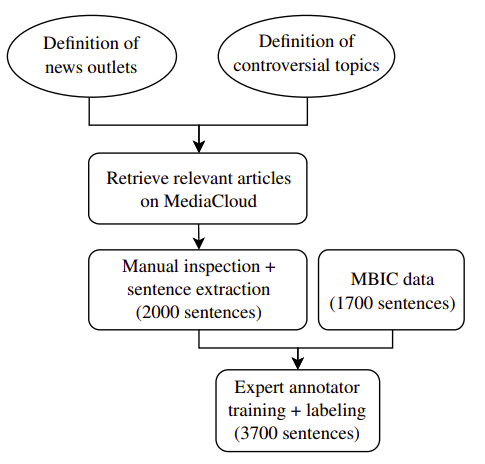
\includegraphics[width=\linewidth]{my_modules/multimedia/babe.png}
  \caption{Data collection and annotation pipeline}
  \label{fig:babe-data}
  \cite{Spinde2021f}
\end{figure}

\section{Wikipedia NPOV datasets}\label{wiki-npov}
Due to annotation costs and the overall lack of large-scale datasets in media bias settings, many researches \cite{pryzant2020automatically,recasens2013linguistic,hube2019neural} used Wikipedia's \Gls{npov} policy\footnote{\url{https://en.wikipedia.org/wiki/Wikipedia:Neutral_point_of_view}}. to construct large-scale datasets automatically. 

Wikipedia's NPOV policy is a set of rules which aim to preserve neutrality in Wikipedia texts. Some examples of NPOV principles are:
\begin{itemize}
    \item Avoid stating opinions as facts.
    \item Avoid stating facts as opinions.
    \item Prefer nonjudgmental language.
\end{itemize}
When neutrality is contested, Wikipedia article can be moved to NPOV dispute by tagging it with \{\{NPOV\}\} or \{\{POV\}\} template. Debate on specific details of neutrality violations is then initialized among editors and eventually resolved, leading to removal of the tag.

This bias information can be used to extract parts of text, that violates NPOV and their unbiased counterparts. However, it has been shown \cite{hube2019neural,zhong-etal-2021-wikibias-detecting} that such automatic extraction can suffer from noisy labelling. In some cases \cite{hube2019neural} up to 60\% of data points were unbiased.

Even though these datasets introduce large amount of samples that are highly related to media bias, they are all sampled from Wikipedia's environment, which isn't same as the News environment. 




\subsection{Wiki Neutrality Corpus}\label{wiki}
\Gls{wnc} \cite{pryzant2020automatically} is a parallel corpus of 180k pairs of biased and unbiased sentences. For the collection of the data, \ref{wiki-npov} approach was adopted. The authors crawled revisions of wikipedia from time span 2014 - 2019. Each revision has been processed to check if it contains any variation of \textit{POV} related text in it. This aproach yielded 180k pairs such that sentence before edit is considered biased and modified/added sentence after edit is considered to be neutral/unbiased.
    
In addition to WNC, 385k of sentences which have not been changed during the NPOV dispute were extracted as neutral and for author's research purposes, the subset of WNC corpus, where only one word is changed in biased-unbiased pair, were added.




\subsection{CW-HARD}
Hube et. al \cite{hube2019neural} constructed a dataset based on NPOV, where only revisions with one sentence diff were filtered. However, this leads to a very noisy dataset, thus the authors sampled 5000 sentences and used crowdsourcing to annotate them with bias/unbiased labels. However, the Krippendorffs Alpha agreement score measured only $\alpha = 0.124$ which is considered low. 

After filtering out sentences which annotators labeled with "I dont know" option, the final dataset consists of 1843 statements labeled as biased 3109 labeled as neutral, a total of 4953 sentences.

\begin{table}
\begin{ctucolortab}
\begin{tabular}{c|c|c|c}
 \textbf{Dataset} & \textbf{Size} & \textbf{Annotation} & \textbf{Agreement}\\
 \hline
 \textbf{SUBJ} & 10.000 & automatic & -\\ 
 \hline
 \textbf{MPQA} & 15.802 & annotators & high \\
 \hline
 \textbf{BASIL} &  1.727 & annotators & medium \\ 
 \hline
 \textbf{Ukraine Crisis Dataset} & 2.057 & crowdsourcing & low \\ 
 \hline
 \textbf{NFNJ} & 888 & crowdsourcing & low \\
 \hline
 \textbf{BABE} & 3700 & annotators & medium \\
 \hline 
 \textbf{WNC} & 362.990 & automatic & - \\
 \hline
 \textbf{CW-hard} & 4953 & crowdsourcing & low \\
 \hline 
 \textbf{WikiBias} & 8198 & annotators & high \\
 \hline
\end{tabular}
\end{ctucolortab}
\caption{Comparison of all bias related datasets collected}
\label{table:1}
\end{table}


\subsection{WikiBias}
This is the latest dataset based on Wikipedia. The authors closely follow the approach of WNC \cite{pryzant2020automatically} and extract another parallel wiki corpus of 214k sentences.
To achieve higher quality corpus, 4,099 sentence pairs were randomly sampled and labeled by trained annotators. As a result introduced WikiBias-Manual dataset consists of 3,400 biased and 4,798 neutral sentences annotated with high \gls{iaa} Cohen's $\kappa = 0.734$




\section{Unused datasets}
Several datasets that are related to media bias but not suitable for the media bias detection task.



\subsection{NewsB}
Focused on detecting political party/ideology.




\subsection{IBC}
Is a dataset focused on detectino of ideology. However,it is not publicly available and I was not able to get the dataset from the authors.


\section{Datasets summary}
In this section I introduced all datasets that are publicly available and are more or less related to the media bias detection task. The overview of all datasets and it's properties can be seen in figure \ref{table:1}.
